% =====================================================================
% Path A — 3DV 2027 submission (DRAFT)
% Aligned to https://3dvconf.github.io/2027/author-guidelines/ :
%   * MANDATORY template: "3DV 2027 Author Kit" (ZIP or Overleaf). Papers not
%     using it are auto-rejected. Replace the \documentclass+preamble below
%     with the kit's; keep the body.
%   * Length: 8 pages INCLUDING figures & tables; references unlimited.
%       -> Budget: this draft has 2 full-width figures (fig2, fig3) + 1 wide
%          table. If it overruns, first make fig3 single-column and/or drop
%          the deep-table excerpt (Table 2) into supplementary.
%   * Abstract <= 4000 characters (current ~1150 -- OK).
%   * DOUBLE-BLIND: author is "Anonymous 3DV submission"; keep all
%     acknowledgments/links/supp/code anonymized (no names, no repo URLs).
%   * Dual submission: <20% overlap with concurrent/previous work (Path A is
%     standalone; keep Path B content out). arXiv preprints are allowed.
%   * PDF only, <=50 MB. Supplementary: PDF/ZIP <=200 MB (anonymized code ok).
%   * Deadlines: paper Aug 28 2026; supp Sep 2 2026; notification Dec 2 2026.
% Figures (same directory): PATHA_fig1_complementarity.pdf,
% PATHA_fig2_method.pdf, PATHA_fig3_qualitative.pdf
% All numbers: seed 20, all scenes per dataset, post-BA, degrees.
% =====================================================================
\documentclass[10pt,twocolumn,letterpaper]{article}
% The 3DV 2027 Author Kit is CVPR-derived (uses cvpr.sty with a review ruler).
% Obtain cvpr.sty from the Author Kit ZIP / Overleaf and place it on the path.
% Use [review] for submission (adds the line ruler + Paper ID); swap to the
% kit's final option for camera-ready. Do NOT alter margins (auto-reject).
\usepackage[review]{cvpr}                 % <-- from the 3DV 2027 Author Kit
\usepackage{times}
\usepackage{graphicx,amsmath,amssymb,booktabs,multirow,xcolor}
\usepackage[pagebackref,breaklinks,colorlinks]{hyperref}
\def\confName{3DV}
\def\confYear{2027}
\newcommand{\mad}{\textsc{madweight}}
\renewcommand{\deg}{^{\circ}}             % degree symbol in math mode
% Required by the author-kit cvpr.sty in [review] mode.
\def\paperID{*****}

\title{When to Remove and When to Reweight:\\
Contamination-Dependent Outlier Handling in Deep Structure-from-Motion}
\author{Anonymous 3DV submission\\ Paper ID *****}

\begin{document}
\maketitle

\begin{abstract}
State-of-the-art deep equivariant Structure-from-Motion (SfM), RESfM, handles outlier
correspondences with a \emph{supervised} inlier/outlier classifier trained on COLMAP-derived
labels. We present \textbf{U-ESFM}, an \emph{entirely self-supervised} alternative: its
outlier head is trained with an adaptive confident-pseudo-label loss (from percentiles of the
model's own reprojection error), and removal, reweighting, robust bundle adjustment, and
per-scene fine-tuning use \emph{no} ground-truth or COLMAP outlier labels. Within this
self-supervised setting we show the \emph{optimal} outlier-handling mechanism is not fixed but
\emph{depends on the scene's contamination level}, and that U-ESFM matches or beats the
COLMAP-supervised classifier exactly where supervision is weakest. Under a strictly controlled protocol---identical point tracks, robust bundle
adjustment, and training schedule, varying only the outlier mechanism---we compare hard
removal, soft reweighting, a three-band hybrid, and a new MAD-remove\,+\,head-reweight
variant (\mad{}) against a from-scratch RESfM baseline across five datasets spanning
$2\%$--$61\%$ measured outliers. We find a clear complementarity: hard, statistics-based
removal wins the high-contamination regime---on an extreme $\sim\!60\%$-outlier held-out
set our label-free \mad{} beats both the supervised baseline ($12.2\deg$ vs.\ $16.2\deg$
translation) and COLMAP itself, which fails to register a third of the cameras; soft
reweighting wins the low-contamination regime, beating the supervised baseline
$2.6$--$3.8\times$ on out-of-distribution BlendedMVS; and in distribution the
self-supervised arms reach mean-level parity with the supervised classifier
($0.316\deg$ vs.\ $0.344\deg$ on MegaDepth), which retains the better median. We attribute
this to domain shift and to a \emph{measurable label ceiling}: regenerating supervision with
from-scratch COLMAP, label recall collapses from $0.82$ to $\sim\!0.3$ and label coverage
from $99\%$ to $\sim\!55\%$ once contamination exceeds $\sim\!15\%$---precisely the regime
where robustness is needed---and we position label-free adaptivity as a missing ingredient
for robust deep SfM.
\end{abstract}

\section{Introduction}
Structure-from-Motion (SfM) recovers camera poses and 3D structure from unordered image
collections. Its correspondences are heavily contaminated by outliers---wrong matches
that survive pairwise geometric verification---particularly in Internet photo collections
where repeated and symmetric structure produces spurious epipolar geometries. Classical
pipelines reject outliers with RANSAC and robust bundle adjustment (BA); recent deep
equivariant methods (ESFM~\cite{esfm}, RESfM~\cite{resfm}) instead learn a
\emph{sets-of-sets} permutation-equivariant network that regresses cameras from point
tracks and, in RESfM, adds a supervised per-point \emph{inlier/outlier classification
module}. RESfM's labels are derived from a COLMAP~\cite{colmap} reconstruction in two
stages: first by track membership, then refined by a $4$-pixel reprojection test against
COLMAP-pose triangulation~\cite{resfm}.

We take a different route. Rather than supervise the head with COLMAP labels, \textbf{U-ESFM}
trains it \emph{self-supervised} --- an adaptive confidence-weighted loss forms confident
pseudo-labels from percentiles of the model's own reprojection error --- so no ground-truth or
COLMAP outlier labels are used anywhere in training or test. On top of this self-supervised
head we study a question RESfM's single supervised mechanism leaves open: \emph{is one
outlier-handling mechanism optimal across the range of contamination levels SfM encounters?}
We find that it is not. Holding everything else fixed---tracks, robust BA, training schedule,
seed---and varying \emph{only} the outlier-handling mechanism, the best mechanism
\textbf{flips with contamination}: aggressive statistics-based removal in the
high-contamination regime, soft reweighting in the low-contamination regime, and the
supervised classifier in the clean, in-distribution regime (Fig.~\ref{fig:complement}).
We further show that a \emph{label-free} removal mechanism---\mad{}, which discards points
by the median-absolute-deviation (MAD) of their reprojection error and soft-weights the
survivors---is the strongest arm at extreme contamination ($\sim\!60\%$ measured outliers),
beating both the supervised from-scratch baseline and COLMAP itself. We attribute this to
(i)~domain shift---the classifier is trained only on in-distribution MegaDepth---and
(ii)~supervised labeling's dependence on a COLMAP reconstruction and ground-truth poses,
readily obtained for curated data but not for the contaminated collections where
robustness is most needed---so a label-free, per-scene mechanism is attractive precisely
in that regime.

\noindent\textbf{Contributions.}
(1)~\textbf{U-ESFM, an entirely self-supervised outlier-handling approach} for deep SfM: an
adaptive confident-pseudo-label head (trained on percentiles of the model's own reprojection
error), label-free statistical removal, and robust BA --- using \emph{no} ground-truth or
COLMAP outlier labels, in contrast to RESfM's COLMAP-supervised head. It matches or beats the
COLMAP-supervised baseline in the high-contamination regime.
(2)~A controlled study of four outlier mechanisms (remove / weight / hybrid / \mad{}),
each with and without test-time fine-tuning, under an identical
tracks\,+\,BA\,+\,schedule pipeline, isolating the mechanism alone.
(3)~The complementarity finding: the optimal mechanism flips with contamination; no single
mechanism dominates.
(4)~\mad{}, which removes outliers by robust reprojection statistics (MAD) --- needing not
even the head --- and reweights survivors; it is the strongest arm at extreme
contamination, beating the from-scratch supervised baseline by $25\%$ translation\,/\,$37\%$
rotation and COLMAP itself at $\sim\!60\%$ measured outliers.

\section{Related Work}
\textbf{Deep equivariant SfM.} Learning-based SfM regresses cameras from point tracks with
permutation-equivariant networks. ESFM~\cite{esfm} casts uncalibrated SfM as deep projective
factorization over a measurement tensor, trained with an unsupervised reprojection loss;
GASFM~\cite{gasfm} uses a graph-attention variant. Both assume outliers were already removed
by two-view geometric verification. RESfM~\cite{resfm} targets contaminated internet
collections with a \emph{sets-of-sets} permutation-equivariant architecture plus a supervised
per-point inlier/outlier classification module and a robust BA, reporting accuracy close to
its own clean-track upper bound (ESFM applied to outlier-free tracks, ``ESFM$^\ast$'') and on
par with classical Theia/GLOMAP. End-to-end pointmap and pose-regression pipelines
(VGGSfM, MASt3R, DUSt3R) target far smaller image sets. Our work proposes no new
architecture; we reuse the RESfM/ESFM backbone and study the outlier-handling stage in
isolation.

\noindent\textbf{Outlier rejection.} Correspondence outliers that \emph{survive} RANSAC/
two-view filtering---from repetitive structure, wide viewpoint, and illumination
change---are the central difficulty in internet-scale SfM. Classical pipelines suppress
them with M-estimators and robust BA; RESfM casts rejection as supervised classification. We
contrast supervised classification against \emph{label-free} statistical removal via the
median absolute deviation (MAD)~\cite{mad} and against soft reweighting, and show their
relative merit is contamination-dependent.

\noindent\textbf{Robust bundle adjustment.} Following~\cite{resfm}, we apply a robust BA
that removes high-reprojection and low-visibility points, keeps the largest connected
component, re-triangulates, and re-optimizes. This stage is identical across all our arms.

\noindent\textbf{Test-time adaptation.} Per-scene fine-tuning at inference is used by ESFM/
RESfM to reach sub-pixel accuracy. We treat it as an orthogonal option ($\pm$TTT) applied
uniformly across mechanisms.

\section{Method}
\subsection{Background}
The input is a (sparse) point-track tensor $M$ of $m$ tracks across $n$ cameras, built by
concatenating pairwise RANSAC-verified SIFT matches. The sets-of-sets permutation-equivariant
network~\cite{resfm,esfm} maps $M$ to per-camera poses and a \emph{per-point} outlier score
$s\in[0,1]$ (points in the same track may receive different scores). Crucially, unlike RESfM
--- whose classification head is trained with a BCE loss against \emph{COLMAP-derived}
inlier/outlier labels --- U-ESFM trains this head \emph{self-supervised}, with an adaptive
confidence-weighted loss: per forward pass it forms confident pseudo-labels from percentiles
of the model's own reprojection error (lowest $p$\% inliers, highest $p$\% outliers) and
applies BCE only to those. No ground-truth or COLMAP outlier labels are used at any point.
A reprojection error $e$ is available for every observation once an initial reconstruction
exists. All mechanisms below consume $s$ (and, for \mad{}, $e$),
produce a per-observation weight $w$ (or a hard keep/drop decision), and feed the result to
the identical robust-BA stage (Fig.~\ref{fig:method}).

\subsection{Outlier-handling mechanisms}
We compare four mechanisms, illustrated as weight-vs-signal transfer functions in
Fig.~\ref{fig:method}:
\begin{itemize}\itemsep2pt
\item\textbf{remove} (the RESfM analogue): drop a point if $s>\tau$; keep with $w{=}1$
otherwise. We use RESfM's default $\tau{=}0.6$ and its $\tau{=}0.8$ for the low-outlier,
single-camera Strecha/BlendedMVS sets~\cite{resfm}.
\item\textbf{weight}: soft, $w=1-s$, no removal.
\item\textbf{hybrid}: three-band---keep ($s$ below a low percentile), soft-weight (middle),
drop ($s$ above a high percentile).
\item\textbf{\mad{}} (ours): removal is driven by robust \emph{reprojection} statistics, not
the head. An observation is removed if its reprojection error exceeds
$\mathrm{med}(e)+\alpha\cdot\mathrm{MAD}(e)$ ($\alpha{=}2$); surviving observations are
soft-weighted by $w=1-s$. \mad{} is the only mechanism that consumes the reprojection
branch $e$ and requires \emph{no} learned threshold for removal.
\end{itemize}
Each mechanism is evaluated with and without test-time fine-tuning ($\pm$TTT), in which the
head continues to adapt on the test scene.

\subsection{Test-time fine-tuning and robust BA}
We load a multi-scene checkpoint, run a per-scene forward pass to obtain $s$ and $e$, apply
the mechanism, fine-tune per scene ($\sim\!1000$ iterations) under the reprojection
objective, and apply robust BA. This protocol, the seed, and the schedule are held fixed
across all arms; only the mechanism block changes.

\section{Experiments}
\subsection{Datasets and contamination}
We evaluate on five datasets spanning a wide contamination range. Alongside the RESfM
paper's quoted outlier fractions we report the contamination \emph{measured on our own
tracks} (robust ground-truth-pose triangulation with the standard $4$px cutoff, applied
uniformly to every dataset):
\begin{center}\footnotesize
\setlength{\tabcolsep}{3pt}%
\begin{tabular}{lccc}
\toprule
Dataset & Out\% (RESfM) & Out\% (ours) & Regime\\
\midrule
Strecha & 2.7 & 1.7 & clean, LIDAR GT\\
BlendedMVS & 3.6 & 3.1 & low-outlier, rendered\\
MegaDepth & 25.6 & 25.4 & contam., \emph{in-dist.}\\
1DSfM & 31.9 & 43.3 & contam., OOD\\
1DSfM-hard & -- & $\sim$60 & extreme, OOD\\
\bottomrule
\end{tabular}
\end{center}
On MegaDepth---where tracks are identical to RESfM's---the two measurements agree
($25.4$ vs $25.6$), validating our measurement; our 1DSfM rebuild is markedly harder than
the tracks behind RESfM's quoted $31.9\%$, which should be kept in mind when reading the
1DSfM columns. \emph{1DSfM-hard} comprises the five 1DSfM scenes unused by the standard
ten-scene split (Gendarmenmarkt, Piccadilly, Roman Forum, Trafalgar, Union Square), built
with the same pipeline and subsampled to $300$ cameras per scene following RESfM's
convention. Networks are trained on 27 MegaDepth scenes; MegaDepth test is therefore
in-distribution, while 1DSfM/Strecha/BlendedMVS/1DSfM-hard are cross-dataset
(out-of-distribution).

\subsection{Protocol, baselines, and track provenance}\label{sec:protocol}
Following RESfM's public training code and default configuration, all networks train for
$20{,}000$ epochs with seed $20$ (the seed reported by RESfM~\cite{resfm}); batch size,
image subsampling, the eleven-milestone learning-rate decay schedule
($10\mathrm{k},11\mathrm{k},\dots,20\mathrm{k}$, $\gamma{=}0.9$), and validation-based
early stopping follow that released configuration and are held identical across all arms.
Two deliberate settings are disclosed. First, the \emph{base} learning rate is per-method:
$10^{-3}$ for the supervised arms (RESfM's released value) and $10^{-4}$ for the
self-supervised arms, whose adaptive pseudo-label loss converges early (best checkpoint by
epoch ${\sim}7.5$k, \emph{before} the first decay milestone; the supervised arms peak at
epoch ${\sim}16.5$k)---both well within the budget, so neither method is
truncation-limited. Second, two secondary values (the infinity-point margin and the
validation metric used for checkpoint selection) are held \emph{identical across all arms}
rather than at RESfM's released values, preserving the controlled comparison. We report two
architectures: shallow ($1{\times}3$) and deep ($2{\times}3$).

\noindent\textbf{Fair-comparison anchor.} Our controlled baseline is
\emph{RESfM-from-scratch}: trained by us with the \emph{identical} setup as our arms (same
27 scenes, sampling, epochs, seed), so only the outlier mechanism differs. We additionally
report \emph{RESfM-released} (authors' weights) and \emph{RESfM (paper)}.\footnote{The
ESFM row likewise follows the unified $20$k-epoch protocol. ESFM's own released
multi-scene (calibrated) recipe trains for $30$k epochs plus a $500$-epoch per-scene
fine-tune; we deliberately hold the schedule fixed across all rows so that the outlier
mechanism remains the only controlled variable.}

\noindent\textbf{Track provenance.} MegaDepth tracks, preprocessing, and the 36 test scenes
are \emph{identical} to RESfM, so MegaDepth is directly comparable to published numbers. The
OOD tracks (1DSfM/Strecha/BlendedMVS) are \emph{reconstructed by us} (RESfM did not release
OOD tracks); OOD comparisons are therefore \emph{controlled within our pipeline} and are
\textbf{not} directly comparable to RESfM's published OOD numbers. On MegaDepth, RESfM's
own released weights yield $0.209\deg$ in our harness (vs.\ their reported $0.169\deg$),
confirming our evaluation is faithful and that $\sim\!0.209\deg$ is the reproducible level;
this is unchanged ($0.217\deg$) under the authors' exact pinned software stack (MKL BLAS,
same pycolmap/pyceres), isolating the residual gap to solver/hardware-level
nondeterminism in robust BA (analysis in the supplementary material).

\noindent\textbf{Training generations.} An earlier generation of our runs used a
five-milestone decay variant ($10\mathrm{k},12\mathrm{k},\dots,18\mathrm{k}$)---an
accidental deviation from RESfM's release, since corrected. The main comparison
(Table~\ref{tab:main}) uses the RESfM-aligned schedule throughout; the wider mechanism
matrix (Table~\ref{tab:shallow}) and the mechanism-level ablations come from the earlier
generation and are labeled as such. A three-seed replication of \emph{both} schedules
shows the schedule effect lies within seed noise (MegaDepth $0.46\pm0.08$ vs.\
$0.40\pm0.09$; 1DSfM $9.6\pm3.2$ vs.\ $12.2\pm2.4$, per-seed rankings \emph{inverting}
on both, the 1DSfM mean dominated by Tower of London, which swings $2\times$ between
seeds). Mechanism \emph{orderings} are stable across generations; single-seed differences
between generations are seed variance, and we flag below the one comparison this affects
(1DSfM at $43\%$).

\noindent\textbf{A method-isolated comparison, not a SOTA claim.} Because
RESfM-from-scratch shares every pipeline component with our arms and differs only in the
outlier mechanism, it isolates the effect of removing supervision---the same controlled
protocol RESfM itself uses when it re-trains ESFM/GASFM in its own pipeline. We do
\emph{not} claim state of the art: RESfM's \emph{released} checkpoint ($0.209\deg$ on
MegaDepth) is stronger than either from-scratch arm. This reproduction gap stems from the
released weights themselves, not our pipeline---the authors' \emph{own} training code on
our tracks reproduces $0.34$--$0.39\deg$, not $0.209\deg$---so it handicaps the
supervised and self-supervised arms \emph{equally}. We report RESfM-released and
RESfM~(paper) as reference rows throughout.

\noindent\textbf{Metrics.} We report mean and median translation and rotation error in
degrees, post-BA. On 1DSfM the mean is dominated by two symmetric-structure failure scenes
(Ellis Island, Tower of London) that fail for \emph{all} methods; we therefore report the
median as the representative figure.

\begin{figure}[t]
\centering
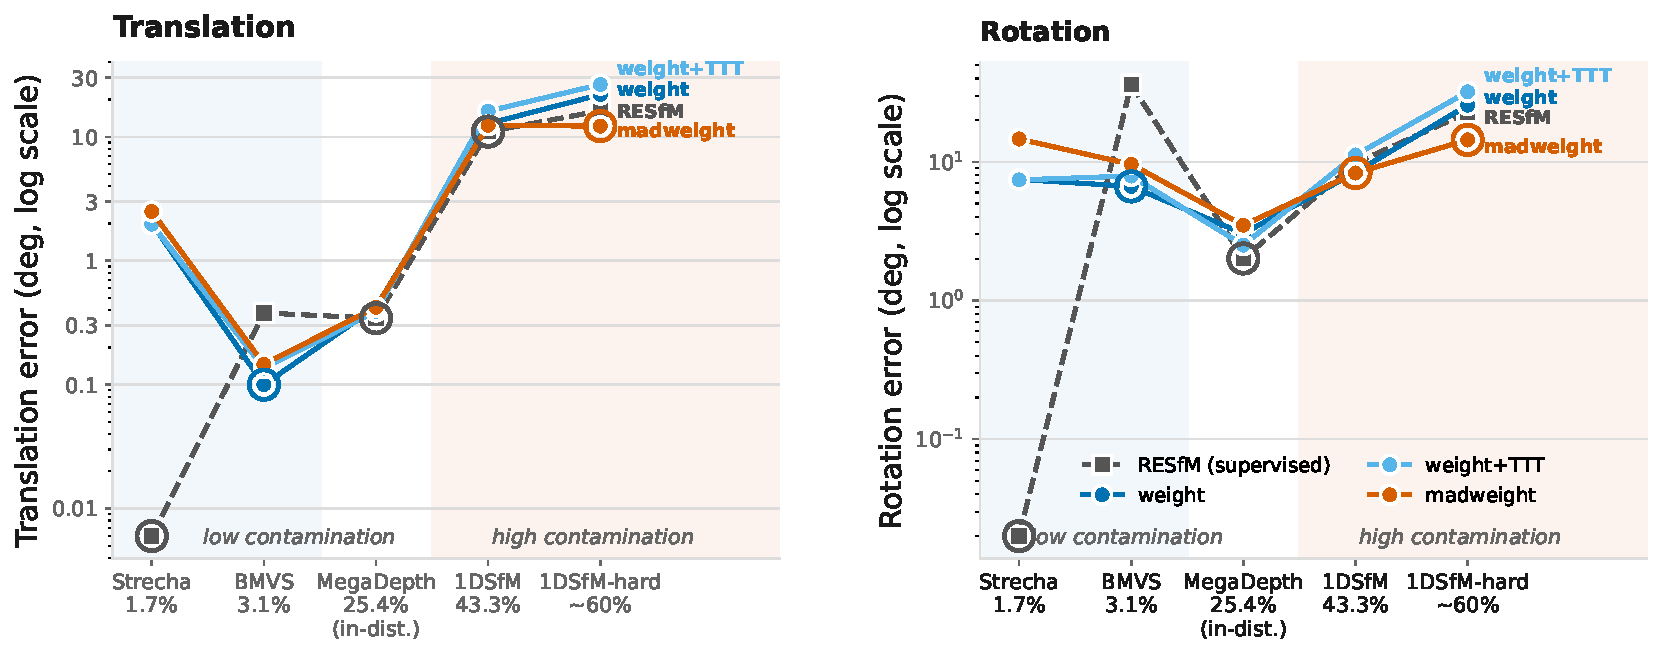
\includegraphics[width=0.88\linewidth]{PATHA_fig1_complementarity.pdf}
\caption{\textbf{The optimal outlier mechanism flips with contamination.} Translation error
(log scale) of U-ESFM's soft \textbf{weight} and \textbf{\mad{}} (both self-supervised) vs.\
COLMAP-supervised RESfM across the four datasets ordered by contamination. Circled point = best per dataset. \mad{} wins
high-outlier 1DSfM; weight wins low-outlier BlendedMVS; RESfM wins clean Strecha and
in-distribution MegaDepth.}
\label{fig:complement}
\end{figure}

\begin{figure*}[t]
\centering
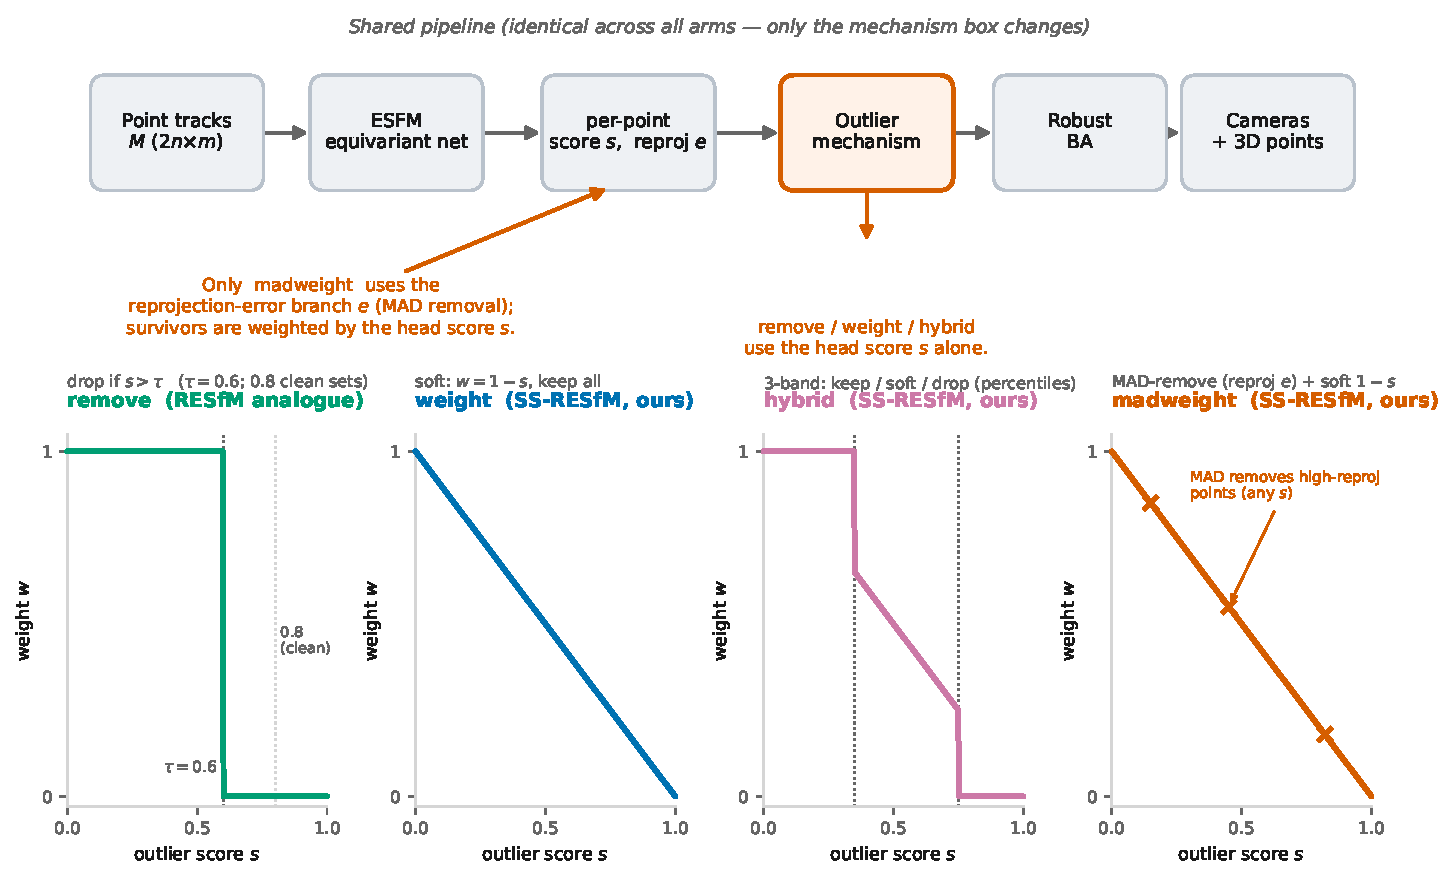
\includegraphics[width=0.85\textwidth]{PATHA_fig2_method.pdf}
\caption{\textbf{Method.} A shared pipeline (top) in which only the outlier-mechanism block
changes. The four mechanisms as weight-vs-signal transfer functions (bottom). Only \mad{}
consumes the reprojection-error branch $e$ for removal; the others use the head score $s$.}
\label{fig:method}
\end{figure*}

\section{Results}
\subsection{Main comparison}
Table~\ref{tab:main} is the controlled head-to-head under the RESfM-aligned schedule:
every row shares tracks, architecture, schedule, robust BA, and seed; only the
outlier-handling mechanism (and its supervision) differs. Four observations.
(1)~\emph{In distribution}, the self-supervised weight+TTT arm attains the better
MegaDepth \emph{mean} ($0.316$ vs.\ $0.344$), while supervised RESfM retains the better
\emph{median} ($0.07$ vs.\ $0.19$)---mean-level parity without labels, with the supervised
head still better on the typical scene. (2)~\emph{Clean OOD splits}: on BlendedMVS every
self-supervised arm beats RESfM by $2.6$--$3.8\times$ ($0.10$--$0.15$ vs.\ $0.38$); on
Strecha RESfM's mean is far better ($0.006$ vs.\ $\sim\!2$), but the medians \emph{tie}
($0.005$)---the self-supervised mean is dominated by a single failure scene.
(3)~\emph{Extreme contamination} ($1$DSfM-hard, ${\sim}60\%$): label-free \mad{} wins
clearly ($12.2$ vs.\ $16.2$), and the soft arms fall behind removal---the regime flip
detailed below. (4)~\emph{Moderate-contaminated 1DSfM} ($43\%$) has no stable winner:
RESfM leads at this seed ($11.0/2.9$ vs.\ \mad{}'s $12.4/4.4$), the earlier generation
showed the reverse ($5.5/2.3$ vs.\ $11.1/4.0$), and the three-seed replication brackets
both---so we decline a directional claim at $43\%$ and rest the high-contamination case
on the $60\%$ set, where the ranking is generation-consistent. The wider eight-mechanism matrix (Table~\ref{tab:shallow}) reports all arms;
the deep-architecture excerpt is in the supplementary material.

\begin{table*}[t]\centering\small
\caption{\textbf{Main controlled comparison (RESfM-aligned schedule).} Mean\,/\,median
translation error (deg, post-BA), seed 20. All rows share tracks, architecture, schedule,
robust BA, and seed; only the outlier mechanism and its supervision differ. Reference rows
(means) below the rule. Best per column in \textbf{bold}.}
\label{tab:main}
\setlength{\tabcolsep}{4.5pt}%
\begin{tabular}{lccccc}
\toprule
Arm & MegaDepth (25.4) & 1DSfM (43.3) & 1DSfM-hard ($\sim$60) & Strecha (1.7) & BlendedMVS (3.1)\\
\midrule
U-ESFM $\cdot$ \mad{}       & 0.422/0.145 & 12.39/4.37 & \textbf{12.21/8.83} & 2.50/0.97 & 0.146/\textbf{0.004}\\
U-ESFM $\cdot$ weight       & 0.423/0.182 & 12.79/11.01 & 21.94/13.13 & 2.00/0.026 & \textbf{0.100}/0.036\\
U-ESFM $\cdot$ weight+TTT   & \textbf{0.316}/0.186 & 16.13/7.16 & 26.44/17.67 & 1.98/\textbf{0.005} & 0.136/0.011\\
RESfM-scratch (supervised)  & 0.344/\textbf{0.070} & \textbf{11.03/2.93} & 16.22/13.08 & \textbf{0.006/0.005} & 0.379/0.348\\
\midrule
RESfM (released)            & 0.209 & 10.71 & -- & 0.197 & 0.330\\
RESfM (paper)               & 0.169 & -- & -- & -- & --\\
\bottomrule
\end{tabular}
\end{table*}

\begin{table*}[t]\centering\small
\caption{\textbf{Full shallow ($1{\times}3$) mechanism matrix} (earlier five-milestone
generation; mechanism orderings are schedule-stable, \S\ref{sec:protocol}). Mean
translation\,/\,rotation error (deg). Dataset headers show RESfM-quoted Outliers\%. Best
U-ESFM per column in \textbf{bold}.}
\label{tab:shallow}
\begin{tabular}{lcccc}
\toprule
Arm & MegaDepth (25.6) & 1DSfM (31.9) & Strecha (2.7) & BlendedMVS (3.6)\\
\midrule
U-ESFM $\cdot$ MAD          & 0.490/4.83 & 6.787/7.48 & 2.807/12.21 & 0.205/12.86\\
U-ESFM $\cdot$ remove       & 0.499/3.80 & 9.854/7.03 & 2.871/12.92 & 0.145/10.20\\
U-ESFM $\cdot$ remove+TTT   & 0.392/3.52 & 10.002/6.82 & 2.768/13.63 & 0.155/9.40\\
U-ESFM $\cdot$ weight       & 0.460/3.97 & 15.884/9.25 & \textbf{1.945}/7.44 & 0.114/6.80\\
U-ESFM $\cdot$ weight+TTT   & 0.527/3.34 & 15.643/7.80 & 2.024/7.41 & 0.126/7.77\\
U-ESFM $\cdot$ hybrid       & 0.463/3.50 & 16.803/7.01 & 3.116/14.84 & 0.124/7.09\\
U-ESFM $\cdot$ hybrid+TTT   & 0.512/4.28 & 17.770/8.72 & 2.229/12.92 & 0.139/8.96\\
U-ESFM $\cdot$ \mad{}       & 0.511/3.72 & \textbf{5.502/5.62} & 2.660/12.02 & \textbf{0.121}/7.80\\
\midrule
RESfM-scratch (ours)        & 0.332/1.60 & 11.067/9.89 & 0.006/0.02 & 0.389/37.64\\
RESfM (released)            & 0.209/1.89 & 11.124/10.59 & 0.197/2.04 & 0.330/31.91\\
ESFM (author)               & 0.756/6.91 & 17.960/14.47 & 1.975/7.35 & 0.227/27.27\\
RESfM (paper)               & 0.169/1.29 & -- & -- & --\\
\bottomrule
\end{tabular}
\end{table*}

\subsection{The complementarity finding}
Fig.~\ref{fig:complement} visualizes the flip on the main-comparison arms. Reading the
per-column winners of Table~\ref{tab:main}, \emph{every dataset is won by a different
arm}: soft weight wins low-outlier BlendedMVS, weight+TTT wins the in-distribution
MegaDepth mean, label-free \mad{} wins extreme 1DSfM-hard, and the supervised classifier
wins clean Strecha (mean) and moderate 1DSfM. The self-supervised wins concentrate exactly
where a label-free design should help---the clean OOD split where the supervised head
misfires on out-of-distribution statistics (BlendedMVS, where RESfM's rotation error also
explodes to $32\deg$), and the extreme-contamination regime where supervision itself can no
longer be manufactured (\S below)---while requiring no COLMAP labels anywhere. Within the
self-supervised arms the removal-vs-weighting ordering is monotone in contamination:
weighting is best at $2$--$3\%$, the two tie in distribution, and removal dominates from
$43\%$ upward ($12.4$ vs.\ $12.8$ at $43\%$; $12.2$ vs.\ $21.9$ at $60\%$)---the
mechanism-level flip that names this paper, stable across both training generations.

\subsection{Why label-free removal wins under high contamination}
Two factors explain why the supervised advantage erodes as contamination rises.
First, \emph{domain shift}: the classifier is trained only on in-distribution MegaDepth,
and its decision boundary does not transfer to the outlier statistics of
out-of-distribution internet collections (a domain-shift effect, not a labeling failure:
the strong in-distribution result confirms the labels are sound). Second, and more
fundamentally, supervision itself degrades in this regime: RESfM's labeling (Appendix~C
of~\cite{resfm}) assumes a COLMAP reconstruction and ground-truth poses per training
scene---readily obtained for curated data, but exactly what one lacks on the contaminated
collections where robustness is most needed. \mad{} requires neither: it recomputes the
outlier test per-scene from reprojection statistics, so it is unaffected by domain shift
and applicable wherever a partial reconstruction exists---which is why it prevails at
extreme contamination.

\paragraph{Measuring the label ceiling.} We make the second argument quantitative. On $18$
scenes spanning the full contamination axis we simulate the realistic labeling scenario for
a \emph{new} dataset---no ground-truth poses, so labels must come from a from-scratch COLMAP
reconstruction of the same tracks (fixed known intrinsics)---and score the resulting
per-observation labels against the ground-truth-pose reference labels
(precision/recall with outlier as the positive class; \emph{coverage} is the fraction of
observations that receive any COLMAP verdict at all, i.e.\ camera registered and track
triangulated; scenes capped at $120$ cameras):
\begin{center}\footnotesize
\setlength{\tabcolsep}{3.5pt}%
\begin{tabular}{lccccc}
\toprule
Contam. & $n$ & Cover\% & Prec. & Recall & COLMAP $t$-err\\
\midrule
0--5\%    & 6 & 99.4 & 0.76 & 0.82 & 0.004\\
5--15\%   & 4 & 89.6 & 0.90 & 0.83 & 0.014\\
15--30\%  & 2 & 71.7 & 0.83 & \textbf{0.26} & 1.02\\
30--45\%  & 3 & 55.7 & 0.74 & \textbf{0.39} & 0.82\\
45--60\%  & 3 & 55.1 & 0.87 & \textbf{0.39} & 11.0\\
\bottomrule
\end{tabular}
\end{center}
Precision stays high throughout, but \emph{recall collapses} from $0.82$ to
$0.26$--$0.39$ and coverage halves once contamination exceeds ${\sim}15\%$: the corrupted
reconstruction absorbs enough outliers that most reproject acceptably under its distorted
geometry, and half the observations receive no label at all. A head trained on such labels
is actively taught that most true outliers are inliers, precisely where robustness
matters. Conversely, below ${\sim}15\%$ COLMAP-derived labels are excellent---consistent
with RESfM's strong in-distribution result and delimiting where the supervised recipe is
sound.

\subsection{Extreme contamination: the 1DSfM-hard set}
To probe beyond 1DSfM's $43\%$, we evaluate on the five held-out 1DSfM-hard scenes
($\sim\!60\%$ measured contamination, $300$ cameras each). All learned arms use the same
controlled protocol as Table~\ref{tab:main} (identical tracks and training generation;
only the mechanism differs)---indeed this column is part of Table~\ref{tab:main}; COLMAP
runs incremental mapping on the same tracks with known intrinsics.
\begin{center}\small
\begin{tabular}{lcc}
\toprule
Method & Trans/Rot (post-BA) & Registered\\
\midrule
U-ESFM $\cdot$ \mad{}      & \textbf{12.2}/\textbf{14.4} & all\\
RESfM-scratch              & 16.2/22.7 & all\\
COLMAP                     & 20.9/--   & 64\%\\
U-ESFM $\cdot$ weight      & 21.9/25.6 & all\\
U-ESFM $\cdot$ weight+TTT  & 26.4/32.0 & all\\
\bottomrule
\end{tabular}
\end{center}
The complementarity extrapolates: label-free removal (\mad{}) beats the
COLMAP-supervised baseline by $25\%$ translation\,/\,$37\%$ rotation, the soft arms fall
further behind, and COLMAP itself degrades severely---its error is computed \emph{only
over the $64\%$ of cameras it registers} (a favorable metric) yet still loses. Errors are
large for every method---these scenes are hard---but the ranking at the extreme matches
the label-ceiling prediction: the supervised advantage inverts exactly where supervision
can no longer be manufactured.

\subsection{Which robust statistic? MAD vs.\ STD vs.\ Huber}
\mad{} removes outliers by a robust statistic of the reprojection error, and the choice of
statistic matters. We ablate the removal criterion while holding the self-supervised head
reweighting fixed (Table~\ref{tab:madstat}): MAD (median${}+\alpha\cdot1.4826\,$MAD; robust,
$50\%$ breakdown), a Huber M-estimate of scale (IRLS), and non-robust STD
(mean${}+\alpha\sigma$), all at $\alpha{=}2$. On heavily-contaminated 1DSfM \textbf{MAD
wins decisively} ($5.50$ vs.\ Huber $10.85$ vs.\ STD $12.26$ mean): the mean/$\sigma$
threshold is inflated by the very outliers it should catch and under-removes, as does
Huber's softer scale, whereas MAD's high-breakdown estimate stays tight. On clean
Strecha/BlendedMVS the ordering reverses---STD's inflated threshold trips on almost
nothing ($\approx$ no removal), the right behavior without outliers; MegaDepth ties
($0.45$--$0.55$). This reinforces the complementarity, and we use MAD in \mad{}.

\begin{table}[t]\centering\small
\caption{\textbf{Removal-statistic ablation} for \mad{} (mean\,/\,median translation, deg;
head reweighting held fixed; five-milestone generation). MAD dominates on contaminated 1DSfM; on clean data the least
aggressive statistic (STD${\approx}$no removal) is best; MegaDepth ties. Best per row in
\textbf{bold}.}
\label{tab:madstat}
\footnotesize\setlength{\tabcolsep}{3.5pt}%
\begin{tabular}{lccc}
\toprule
Dataset & MAD (\mad{}) & Huber & STD\\
\midrule
1DSfM     & \textbf{5.50/2.32} & 10.85/6.56 & 12.26/4.75\\
MegaDepth & 0.511/0.154 & \textbf{0.454}/0.178 & 0.547/0.234\\
Strecha   & 2.66/1.05 & 2.76/1.19 & \textbf{2.07/0.11}\\
BlendedMVS & 0.121/0.047 & 0.183/0.150 & \textbf{0.116/0.002}\\
\bottomrule
\end{tabular}
\end{table}

\subsection{Per-scene complementarity and the limits of contamination-based selection}
The complementarity above is stated at the dataset level. Because individual scenes span
a wide contamination range (1DSfM $29$--$56\%$, MegaDepth $0.2$--$47\%$), we test whether
the flip also holds \emph{per scene}. Fig.~\ref{fig:perscene} plots, for every scene, its
own outlier rate against the signed advantage of removal over soft weighting,
$\log_{10}(\mathrm{err}_{\mathrm{weight}}/\mathrm{err}_{\mathrm{removal}})$. On
out-of-distribution data the trend matches the dataset-level story: soft weight wins the
low-contamination scenes ($6/7$ below $5\%$) and a removal mechanism wins the
high-contamination scenes ($7/8$ above $30\%$). The flip is thus a scene-level phenomenon,
not an artifact of dataset averaging.

Two caveats: the OOD contamination distribution is bimodal ($0.5$--$2.7\%$ vs.\
$29$--$56\%$), so the crossover is only bracketed to $\sim\!3$--$29\%$; and at the clean
end many scenes are near-ties (sub-$0.05\deg$ for every mechanism), so the
low-contamination signal is weak in magnitude even where its sign is consistent.
MegaDepth fills the middle but is in-distribution and removal-dominated throughout.

\begin{figure}[t]
\centering
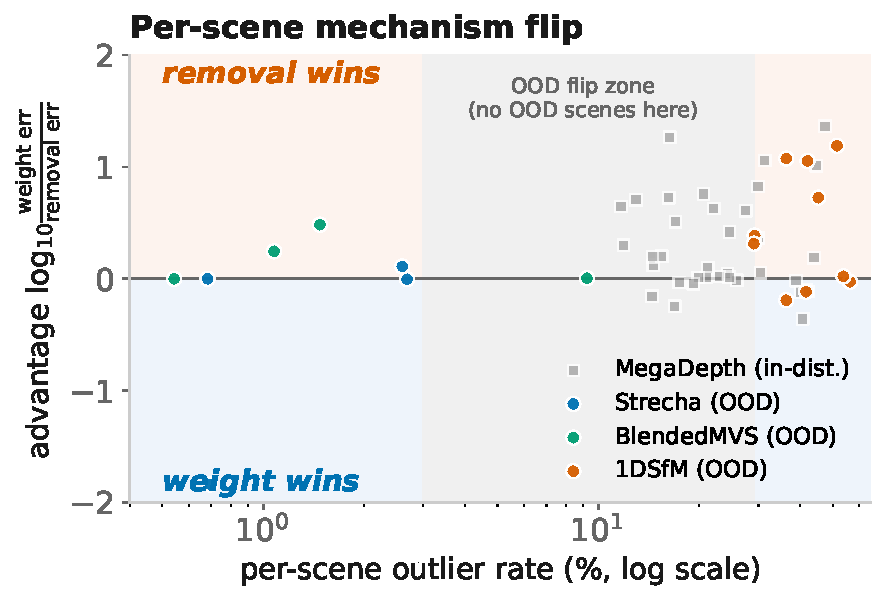
\includegraphics[width=0.88\linewidth]{PATHA_fig4_perscene.pdf}
\caption{\textbf{Per-scene complementarity.} Each point is one scene: its own outlier rate
(x, log) vs.\ the signed advantage of removal over soft weighting. On OOD data (circles),
weight wins at low contamination and removal at high contamination; the crossover lies in
the sparsely-sampled $3$--$29\%$ band. MegaDepth (squares) is in-distribution.}
\label{fig:perscene}
\end{figure}

\begin{table}[t]\centering\small
\caption{\textbf{Per-scene selection} (mean translation, deg; five-milestone
generation). Contamination-keyed
selection (madweight if scene outlier rate ${\ge}10\%$, else weight) does not improve over
per-dataset selection. The last column is an \emph{oracle} that selects the best of the four
mechanisms per scene \emph{using ground-truth error}---an upper bound and headroom analysis,
not a deployable method. It matches RESfM-released on MegaDepth (0.20 vs 0.21) rather than
beating it and still loses Strecha, and the signal it needs is not per-scene contamination;
realizing it without ground truth is left to future work.}
\label{tab:selector}
\footnotesize\setlength{\tabcolsep}{3pt}%
\begin{tabular}{lcccc}
\toprule
Dataset & weight & madwt & contam & oracle (GT)\\
\midrule
MegaDepth  & \textbf{0.459} & 0.511 & 0.511 & \textit{0.204}\\
1DSfM      & 15.89 & \textbf{5.50} & 5.50 & \textit{4.58}\\
Strecha    & \textbf{1.95} & 2.66 & 1.95 & \textit{1.95}\\
BlendedMVS & 0.112 & 0.122 & 0.112 & \textit{0.048}\\
\bottomrule
\end{tabular}
\end{table}

\noindent\textbf{Does per-scene contamination help selection?} Choosing madweight vs.\ weight
\emph{per scene} by its contamination does \emph{not} improve the aggregate
(Table~\ref{tab:selector}): within each dataset the contamination is too homogeneous relative
to any threshold to trigger different choices, so a contamination-keyed selector collapses to
per-dataset selection---and on in-distribution MegaDepth it chooses removal for every scene
and thereby \emph{underperforms} plain weight ($0.51$ vs.\ $0.46$). An \emph{oracle} picking
the best of all four mechanisms per scene (using ground-truth error) would help
substantially---MegaDepth $0.46\!\to\!0.20$ (matching RESfM-released $0.209$) and 1DSfM
$5.50\!\to\!4.58$---but the signal it needs is not per-scene contamination, which separates
datasets rather than scenes within them. A deployable per-scene selector therefore requires a
richer signal than contamination alone; we leave it to future work.

\noindent\textbf{Why a cheap unsupervised selector fails.} Beyond contamination, we tested
three ground-truth-free selection signals against the oracle's per-scene choice on 1DSfM
(10 scenes, four mechanisms): (i)~final reprojection error; (ii)~held-out cross-validation
reprojection (re-triangulate each point from $80\%$ of its cameras, score on the held-out
$20\%$); and (iii)~cycle consistency of the reconstruction's relative rotations against
independent five-point essentials from the raw matches. None recovers the oracle. Both
reprojection proxies are \emph{degenerate}---aggressive removal minimizes any reprojection
metric by retaining only easy points, so they select \texttt{remove} on every scene ($6/10$,
the base rate, carrying no per-scene information), and held-out reprojection is fooled by
self-consistent folded reconstructions---while cycle consistency scores $1/10$: on
contaminated collections the pairwise essentials that would serve as an external reference
are themselves unreliable. Realizing the oracle's headroom thus appears to require a
\emph{learned} selector, which would inherit the very domain-shift limitation that motivates
our self-supervised design. At the regime (per-dataset) level, however, contamination
already selects the right mechanism, which is the practical recommendation we adopt.

\subsection{Threshold sensitivity}
To rule out an under-tuned baseline, we sweep the remove threshold
$\tau\in\{0.4,\dots,0.8\}$ (RESfM searches the same range). The optimum shifts with
contamination---the most contaminated OOD dataset (1DSfM) prefers the most aggressive
$\tau{=}0.4$, the cleanest (BlendedMVS) prefers $\tau{=}0.8$---but the trend is weak and
broken by in-distribution MegaDepth ($\tau{=}0.6$--$0.7$). Crucially (five-milestone
generation), no threshold closes the MegaDepth gap to RESfM-released (best remove
$0.384\deg$ vs.\ $0.209\deg$) and none beats \mad{} on 1DSfM ($7.98\deg$ vs.\ $5.50\deg$).
Threshold tuning improves the remove arm but does not overturn the complementarity
picture.

\subsection{Qualitative}
Fig.~\ref{fig:qual} overlays BA-aligned camera centers on ground truth for 1DSfM
NYC\_Library (five-milestone generation). Label-free \mad{} ($1.32\deg$) leaves far fewer gross-drift cameras than the
supervised from-scratch baseline ($5.42\deg$), whose estimates drift more numerously and
farther.

\begin{figure}[t]
\centering
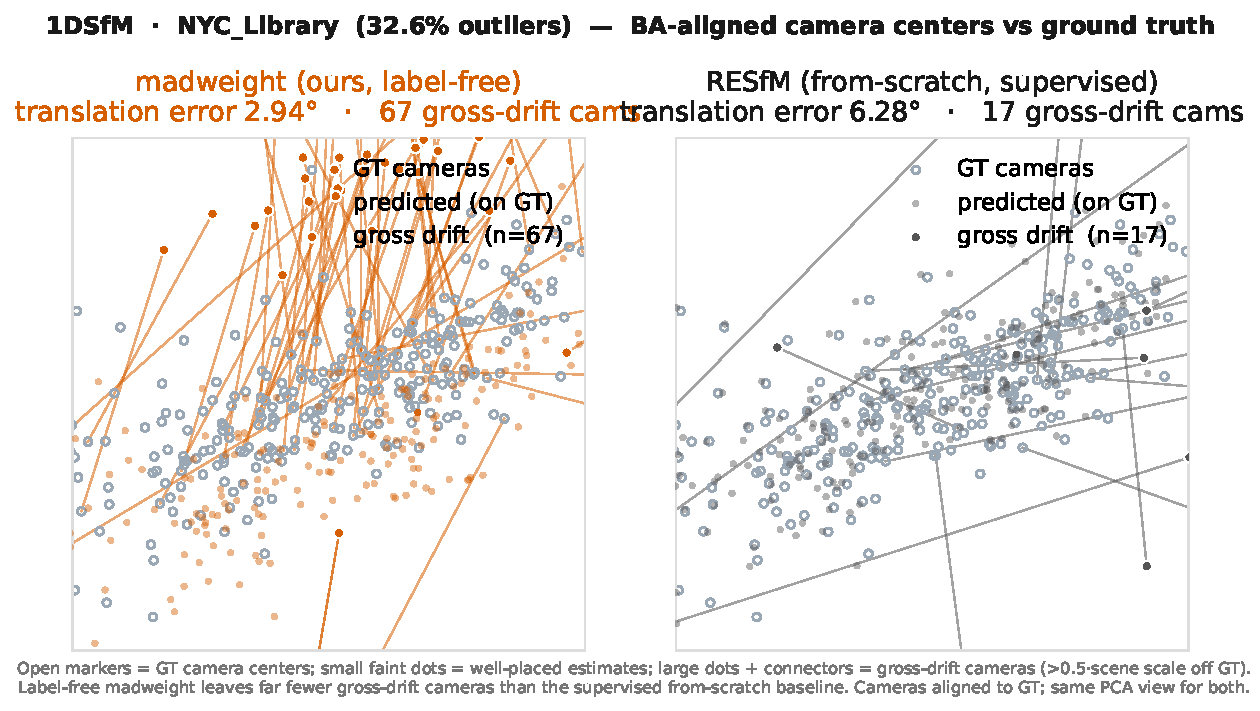
\includegraphics[width=0.86\linewidth]{PATHA_fig3_qualitative.pdf}
\caption{\textbf{Qualitative 1DSfM (NYC\_Library, 32.6\% outliers).} BA-aligned camera
centers vs.\ GT (open markers); large dots\,+\,connectors mark gross-drift cameras. \mad{}
(left, $1.32\deg$) has fewer and shorter drifts than RESfM-from-scratch (right, $5.42\deg$).}
\label{fig:qual}
\end{figure}

\section{Limitations}
(1)~No single deployable configuration wins all datasets; selecting the best mechanism per
dataset (Table~\ref{tab:main}) requires knowing the contamination level. We present a study
of the phenomenon, not a turnkey adaptive method; an unsupervised selector is future work.
(2)~The in-distribution parity is mean-level only: supervised RESfM keeps the better
MegaDepth median and the clean Strecha mean, and RESfM-released remains stronger than
either from-scratch arm on MegaDepth, so we claim no SOTA. (3)~At moderate contamination
($43\%$, 1DSfM) no winner is stable across seeds and training generations; our
high-contamination claim rests on the $\sim\!60\%$ set, where the ranking is consistent.
(4)~OOD tracks are self-constructed; OOD numbers are controlled within our pipeline
and not comparable to RESfM's published OOD numbers. (5)~Two symmetric-structure scenes
(Ellis Island, Tower of London) fail for all methods and inflate 1DSfM means; we report
medians alongside. These are exactly the cases where excess removal can disconnect the
viewing graph---a failure mode RESfM itself reports~\cite{resfm}.

\section{Conclusion}
U-ESFM shows that deep SfM outlier handling can be made \emph{entirely
self-supervised}---with no ground-truth or COLMAP labels---and still reach mean-level
parity in distribution and win the clean-OOD and extreme-contamination regimes. The
optimal mechanism is contamination-dependent: removal wins high contamination (where
label-free \mad{} beats the supervised baseline and COLMAP itself, precisely where
COLMAP-based supervision is hardest to obtain), reweighting wins low, and the supervised
baseline retains the clean and typical-scene regimes. Robust deep SfM should treat outlier
handling as adaptive and self-supervised rather than a single supervised mechanism. Code,
configurations, and the rebuilt OOD tracks will be made publicly available upon
publication.

\label{sec:endcontent}%
\begin{thebibliography}{9}\small

\bibitem{resfm} Khatib, Kasten, Moran, Galun, and Basri. RESfM: Robust Deep Equivariant Structure from Motion. ICLR 2025.

\bibitem{esfm} Moran, Koslowsky, Kasten, Maron, Galun, and Basri. Deep Permutation Equivariant Structure from Motion. ICCV 2021.

\bibitem{gasfm} Brynte, Iglesias, Olsson, and Kahl. Learning Structure-from-Motion with Graph Attention Networks. CVPR 2024.

\bibitem{colmap} Sch\"onberger and Frahm. Structure-from-Motion Revisited. CVPR 2016.

\bibitem{mad} Rousseeuw and Croux. Alternatives to the Median Absolute Deviation. JASA 1993.

\bibitem{onedsfm} Wilson and Snavely. Robust Global Translations with 1DSfM. ECCV 2014.

\bibitem{megadepth} Li and Snavely. MegaDepth: Learning Single-View Depth Prediction from Internet Photos. CVPR 2018.

\bibitem{strecha} Strecha et al. On Benchmarking Camera Calibration and Multi-View Stereo for High-Resolution Imagery. CVPR 2008.

\bibitem{blendedmvs} Yao et al. BlendedMVS: A Large-Scale Dataset for Generalized Multi-View Stereo Networks. CVPR 2020.

\end{thebibliography}

\end{document}
